

\beginsong{Björneborgarnas marsch}[
by={Johan Ludvig Runeberg},
index={Söner av ett folk som blött}]

\beginverse*
Söner av ett folk som blött
på Narvas hed, på Polens sand, på Leipzigs slätter, Lützens kullar,
än har Finlands kraft ej dött,
än kan med oväns blod ett fält här färgas rött.
Bort, bort, vila, rast och fred!
En storm är lös, det ljungar eld och fältkanonens åska rullar;
framåt, framåt led vid led!
På tappre män se tappre fäders andar ned.
Ädlaste mål
oss lyser på vår bana;
skarpt är vårt stål
och blöda är vår vana.
Alla, alla käckt framåt!
Här är vår sekelgamla frihets sköna stråt.
Lys högt, du segersälla fana,
sliten av strider sen en grånad forntids dar,
fram, fram, vårt ädla, härjade standar!
Än finns en flik med Finlands gamla färger kvar!
\endverse
\endsong

\begin{figure}
\begin{center}
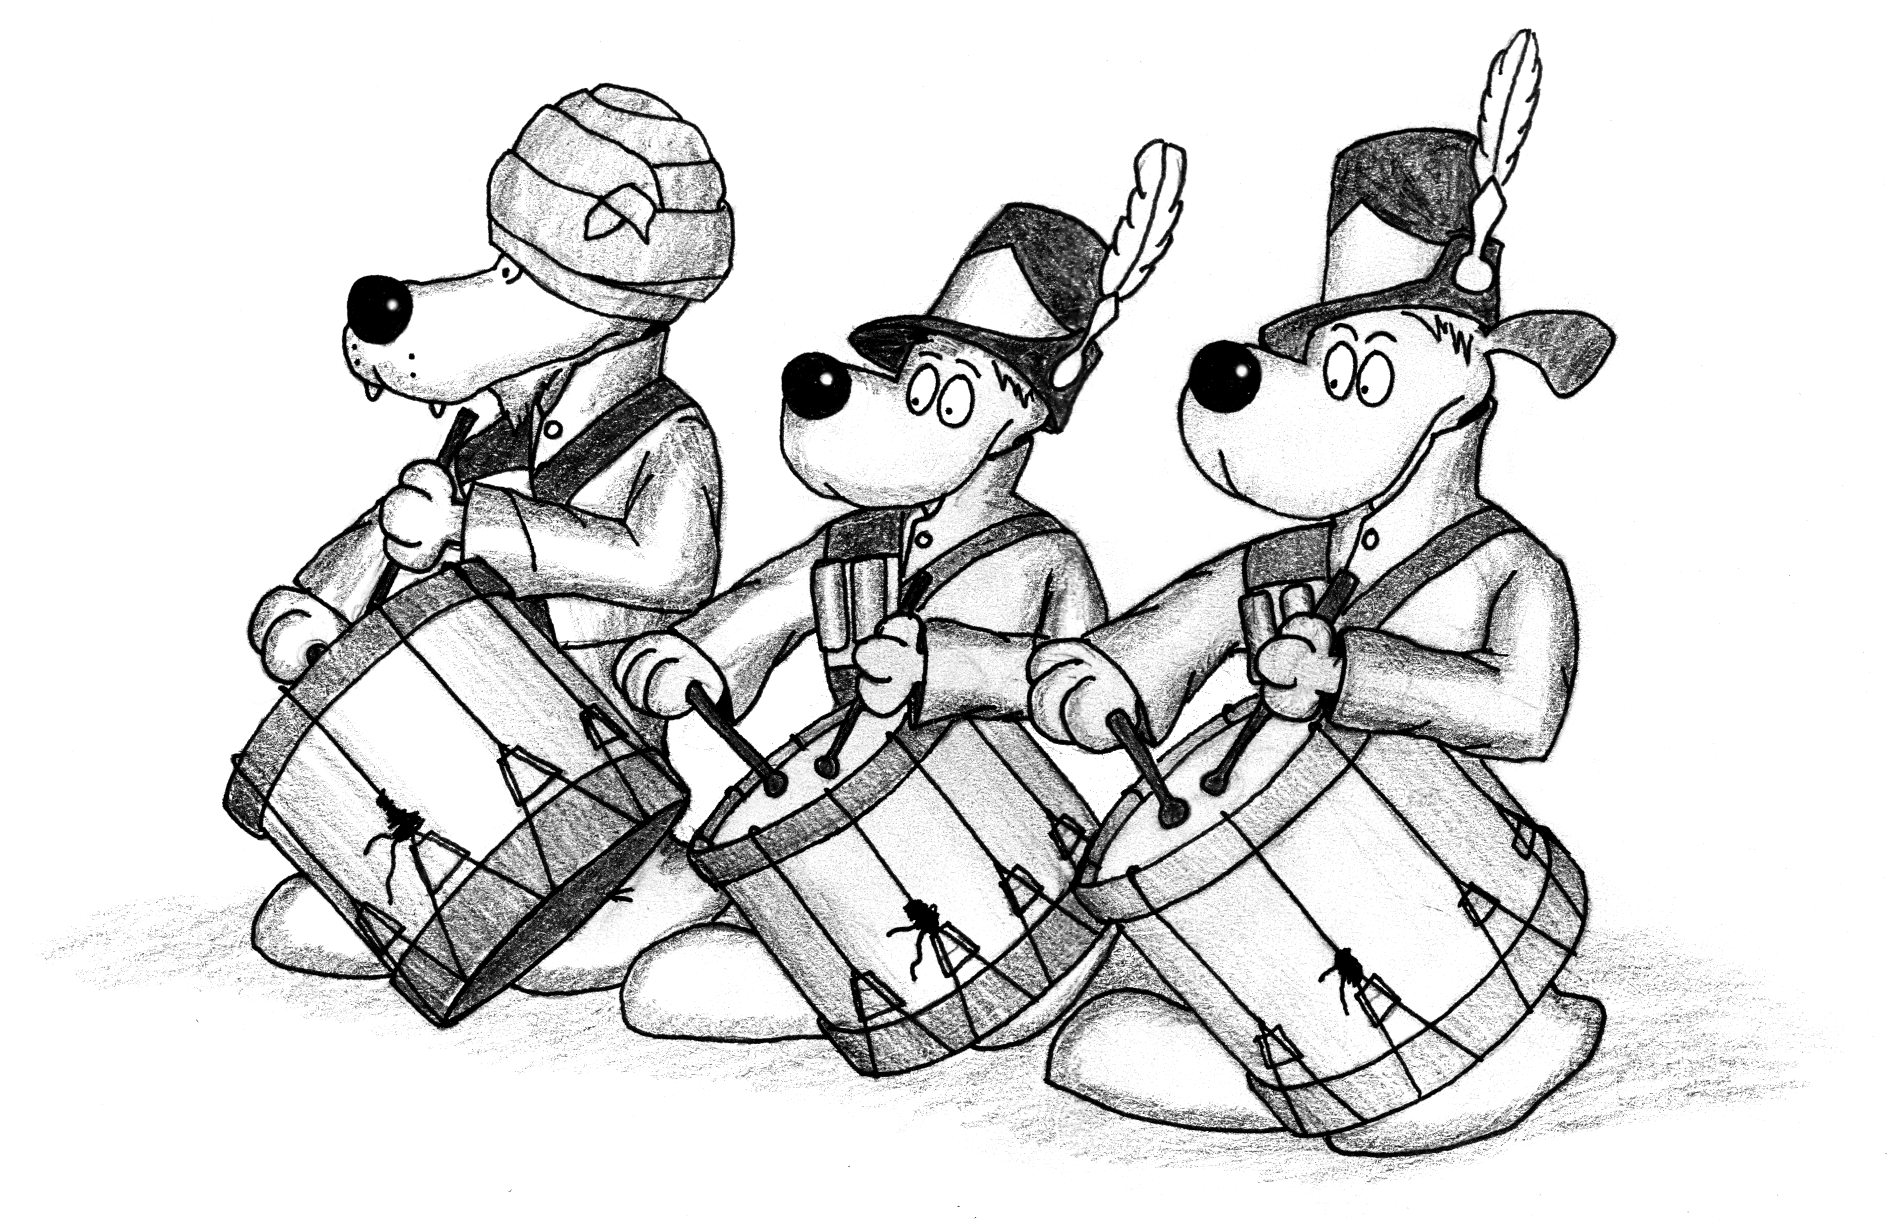
\includegraphics[scale=.5]{../bilder/bjorneborgarnas_marsch.png} 
\end{center}
\end{figure}

